\chapter{Methodology}
\label{chap:methodology}

\section{Overview}
This chapter discusses the methodological approaches considered for developing the Agentic AI Tutor and explains the rationale behind the final design.

\section{Knowledge Integration Techniques Selection}
\subsection{Requirements}

The selected technique must satisfy several requirements:

\begin{enumerate}
    \item \textbf{Maintainability} Course materials change often and should be integrated without retraining.
    \item \textbf{Reduced hallucinations} The system must produce grounded and reliable answers.
    \item \textbf{Explainability} Both students and teachers should be able to trace the source of information.
    \item \textbf{Support for isolated subject modules} The system must allow each subject to function as an independent module so that computational load can be distributed between subjects when necessary and scaling does not affect the rest of the system.
\end{enumerate}

These requirements guide the comparison of RAG, CAG, and fine-tuning.

\subsection{Fine-tuning Only}
Fine-tuning adjusts internal model weights and can produce high accuracy on narrow domains. This process improves task performance but requires large, curated datasets and high computational power. Once trained, the model cannot automatically update its knowledge without repeating the training process \parencite{RAGvsCAG95:online}. Every update to course content requires new datasets, new preprocessing, and repeated training. For educational applications where lecture materials and tutorials are regularly updated, this approach becomes inefficient and costly compared to retrieval-based methods. It also does not reliably reduce hallucinations, because the model may still generate unsupported statements when internal knowledge is insufficient. Fine-tuning offers limited explainability, as the model cannot cite sources after the weights are updated.

\subsection{Retrieval-Augmented Generation}
Retrieval-Augmented Generation (RAG) improves factual accuracy by integrating real-time information retrieval directly into the generation workflow \parencite{RAGvsCAG99:online}. According to \parencite{RAGvsCAG95:online}, RAG combines a retriever and a generator: the retriever searches an external database for documents related to a user query, and the generator then produces an answer that uses both internal and retrieved knowledge. This approach allows a language modals to find up-to-date information before responding, producing answers that are more accurate and context-aware \parencite{RAGvsCAG99:online, 2506059250:online, WhatisRe45:online}.

\parencite{RAGvsCAG99:online, WhatisRe45:online} describes the RAG workflow as a multi-step process. This workflow includes the following steps:
\begin{enumerate}
\item Converting the query into an embedding vector.
\item Searching a vector database for semantically similar context.
\item Appending retrieved context to the query.
\item Generating the final response using both internal and external knowledge.
\end{enumerate} 
These steps ensure that the model selects only the most relevant content and integrates it coherently into its output. RAG therefore reduces hallucinations and improves reliability in knowledge-intensive domains such as education and research.

Conceptually, Retrieval-Augmented Generation (RAG) uses a retriever to fetch semantically similar chunks and a generator to condition on retrieved evidence \parencite{2005114070:online,WhatisRe45:online}. For each subject, a ChromaDB index of slides and notes can be maintained with task-appropriate chunking and retrieval gating to reduce irrelevant retrieved chunks \parencite{ChromaDB63:online}.

RAG complements fine-tuning by enabling rapid knowledge updates without re-training and supports explainability via citation of source passages.

RAG directly supports several key requirements of the project. It enables maintainability by allowing new lecture slides, notes, and examples to be integrated immediately into the system without retraining.  \parencite{2506059250:online} report that small open-weight models (3B-7B parameters) augmented with RAG achieved higher accuracy and lower hallucination rates in teacher-assistant tasks compared with the same models without retrieval. This also improves explainability, as retrieved passages can be cited or displayed to the learner.  Similarly, \parencite{RAGvsCAG99:online} notes that RAG is ideal for tasks requiring factual grounding, document referencing, and dynamic updates, even though retrieval quality and ranking logic may influence latency.

Because each subject maintains its own vector store and retrieval logic, RAG naturally fits the requirement for isolated subject modules. Updates or heavy workloads in one subject do not affect others, and each subject can scale independently based on usage.

\subsection{Cache-Augmented Generation}
Cache-Augmented Generation (CAG) focuses on injecting domain-specific or preloaded context directly into the generation pipeline. It is faster than retrieval-based systems because it skips external searches and uses internal memory \parencite{RAGvsCAG99:online}. This makes it suitable for small, well-defined environments where the context rarely changes \parencite{RAGvsCAG95:online}. However, it does not meet the project's maintainability requirement. Cached content must be updated manually, which becomes impractical when course materials change. It also provides limited protection against hallucinations because the model can still ignore cached context. As \parencite{2506059250:online} note, CAG can assist with stylistic or pedagogical alignment in educational systems but is not a reliable substitute for factual retrieval.

\subsection{Knowledge Integration Techniques Selection Rationale}
Based on the defined requirements, Retrieval-Augmented Generation is the preferred method. It provides fast and low-cost knowledge updates, reduces hallucinations by grounding answers in course materials, and supports transparent explanations through direct citations. RAG also aligns naturally with subject-level isolation, as each subject can maintain its own vector database and retrieval pipeline. Moreover, RAG dynamically accesses updated lecture slides and tutorials stored in vector databases, without requiring new training cycles. This makes it more scalable for courses that evolve over time. In contrast, Cache-Augmented Generation requires manual updates of its cached memory, while fine-tuning must be repeated whenever new material is added. CAG can be used in limited cases where small static context is needed, but it cannot serve as the primary mechanism due to maintainability issues. Fine-tuning is reserved for improving model behaviour or pedagogy, not for encoding factual course content.

Overall, RAG offers the best balance of accuracy, maintainability, explainability, and modularity, and therefore it is selected as the core knowledge integration technique for this system.

\section{Operational Methodologies Selection}
\subsection{Requirements}
The following requirements guide the choice of operational methodology:
\begin{enumerate}
    \item \textbf{Reproducibility} All models and agents must run in predictable and version-controlled environments.
    \item \textbf{Scalability} Each subject module must be able to scale independently, as the system will run separate models for different subjects.
    \item \textbf{Observability} The system must collect logs, metrics, and traces for debugging and for monitoring model drift.
    \item \textbf{Automation} Continuous delivery, validation, and updates should minimise manual intervention.
    \item \textbf{Safety and compliance} Educational systems require strict control over data access, model versions, and auditability.
\end{enumerate}

These requirements inform the comparison of MLOps practices, LLMOps extensions, and traditional Data Science development workflows.

\subsection{Data Science Life Cycle}
The Data Science Life Cycle (DSLC), as formalised in \textcite{TheDataS80:online}, provides a structured view of how data-driven systems evolve through iterative stages of acquisition, preparation, modelling, validation, and dissemination. DSLC is relevant to this project because it emphasises reproducibility, transparency, and the preservation of research artefacts across the entire workflow. These principles support predictable behaviour of subject-specific small language models, especially when they operate on evolving datasets such as updated lecture materials, tutorial solutions, or new assessment examples.

DSLC highlights that each stage generates artefacts: data, code, workflow steps, statistical assumptions, and documentation. That artefacts must be preserved to ensure scientific integrity. For an educational AI system, this is particularly important: datasets and model outputs may be reused, audited, or revalidated, and instructors must be able to trace how outputs were produced.

\begin{figure}[h]
    \centering
    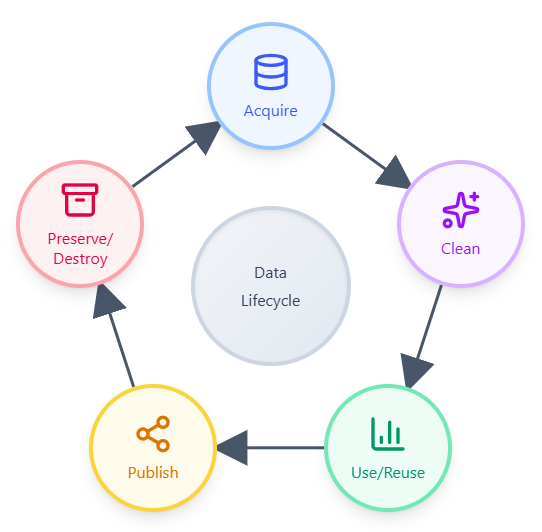
\includegraphics[width=0.85\textwidth]{figs/dslc-diagram.png}
    \caption{Data Science Life Cycle (DSLC) stages, adapted from \textcite{TheDataS80:online}.}
    \label{fig:dslc}
\end{figure}
\FloatBarrier

DSLC further emphasises reproducibility, documentation, metadata creation, and artefact preservation through stages:

\paragraph{DSLC Lifecycle Stages} \textcite{TheDataS80:online}
\begin{itemize}
    \item \textbf{Acquire} Raw data, metadata, and contextual information are collected from relevant sources. Documentation of the acquisition process is preserved to ensure the dataset can be reconstructed and understood.
    \item \textbf{Clean} Data is organised, filtered, annotated, and cleaned. All preprocessing scripts, decisions, and intermediate versions are archived to maintain reproducibility and traceability.
    \item \textbf{Use/Reuse} Cleaned data is analysed, mined, and modelled. Additional derived datasets, visualisations, and decision outputs are generated. All modelling code, training configurations, and computational artefacts are stored to enable reuse and comparative analysis.
    \item \textbf{Publish} Final datasets, code, workflows, and documentation are disseminated. Results are aggregated and coupled with relevant literature. Reusable artefacts are shared through repositories, portals, or databases to support transparency and further research.
    \item \textbf{Preserve/Destroy} Long-term data stewardship decisions are made: data and models may be preserved, replicated, indexed, compressed, curated, or intentionally destroyed. These actions ensure compliance with ethical, regulatory, and sustainability requirements.

\end{itemize}

However, DSLC does not address continuous deployment, real-time inference, large-scale monitoring, or distributed container orchestration. Its lifecycle stages describe how data work should be organised, but do not provide mechanisms for scalable or automated operation of model containers. Therefore, DSLC is essential for governance and reproducibility, but insufficient as an operational methodology for running subject-specific SLMs in production.

\subsection{MLOps}
MLOps focuses on deploying, monitoring, and maintaining machine learning systems in production environments. The empirical study by Amrit and Narayanappa \parencite{Ananalys40:online} \parencite{Ananalys40:online} identifies organisational, technical, and operational challenges in model deployment, including version management, automation, reproducibility, model drift, and workflow complexity. MLOps frameworks address these challenges through CI/CD pipelines, container orchestration, model registries, automated testing, and performance monitoring.

\begin{figure}[h]
    \centering
    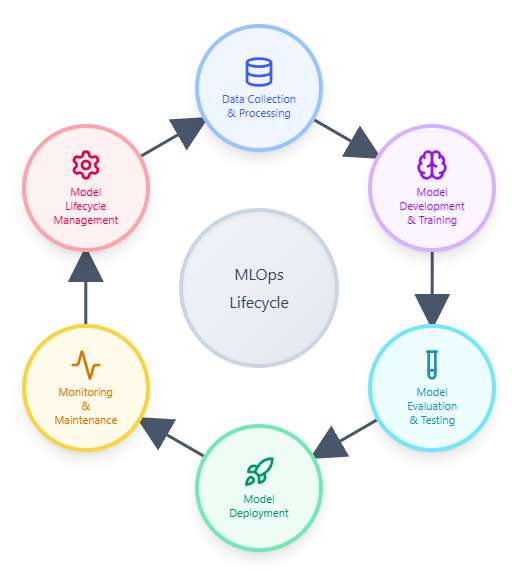
\includegraphics[width=0.85\textwidth]{figs/mlops-diagram.png}
    \caption{MLOps workflow stages, adapted from \textcite{Untitled64:online}.}
    \label{fig:mlops}
\end{figure}
\FloatBarrier

\paragraph{MLOps Lifecycle Stages} \parencite{Untitled64:online}
\begin{itemize}
    \item \textbf{Data collection and processing} Data is gathered from relevant sources and prepared for modelling. This includes cleaning, formatting, transformation, and enrichment steps that ensure the dataset is suitable for training and evaluation.
    \item \textbf{Model development and training} Appropriate algorithms are selected, model architectures are designed, and training routines are executed. During this stage, models are fitted to the processed data and their initial performance is assessed.
    \item \textbf{Model evaluation and testing} Trained models are tested on separate evaluation data to measure accuracy, robustness, and generalisation. Additional checks, such as security, reliability, and compliance tests are carried out to ensure the model is ready for deployment.
    \item \textbf{Model deployment} Models are packaged with their required dependencies and deployed to the intended runtime environment. This may involve containerisation, orchestration, or integration with existing services.
    \item \textbf{Monitoring and maintenance} The deployed model is continuously observed for performance issues, drift, failures, or unexpected behaviour. Alerts and logs help identify when updates, retraining, or corrective actions are needed.
    \item \textbf{Model lifecycle management} All stages: development, deployment, and ongoing operation are coordinated as part of a unified lifecycle. This ensures consistent governance, traceability, and compliance across the entire machine learning workflow.
    
\end{itemize}

MLOps aligns closely with all project requirements. MLOps principles ensure that each subject-specific model runs in a controlled and versioned environment. They also support observability and safety. The system must monitor drift, maintain audit trails, and guarantee that updates do not break existing functionality. MLOps further enables independent scaling of the three models used in this project, ensuring that high demand in one subject does not affect the others.

\subsection{Methodology Selection Rationale}

DSLC offers a strong conceptual structure for reproducibility and documentation, especially regarding artefact preservation from data to publication. However, DSLC is not an operational framework and does not support scalability, automation, or continuous monitoring.

MLOps provides mature, general-purpose operational tools for machine learning systems. It directly supports reproducible deployment, containerisation, CI/CD, monitoring, and access control. MLOps matches all critical requirements and supports the architecture of three independent subject modules, each running its own SLM container. Therefore, MLOps offers the best balance of reliability, maintainability, automation, and scalability for the Agentic AI Tutor system and is chosen as the core operational methodology.

Taken together, the chosen knowledge integration technique (RAG) and the operational methodology (MLOps) define how the Agentic AI Tutor will both access course knowledge and remain robust in production.

The following chapter outlines how these methodological choices are translated into a practical implementation plan to build the Agentic AI Tutor in practice.
